\documentclass{article}
\usepackage{graphicx}
\usepackage{caption}
\usepackage{subcaption}
\usepackage{hyperref}
\graphicspath{{./figs/}}{}
\usepackage{listings}
\title{
HLS-Assignment 9 PART-2
}
\begin{document}

\maketitle
\hfill \textbf{VIVADO-VERILOG}
\section{Problem Statement}
\href{run:./problem_statement.pdf} {Problem Statemt}
\vspace{1cm}

\section{CRC bits Generator Code}
\begin{lstlisting}
//crcaxis.v
`timescale 1ns / 1ps

module axis_reg #(
        parameter integer DW_IN = 8,
        parameter integer DW_OUT = 32
    )
    (
        
        input wire clk,
        input wire reset_n,
        input wire [DW_IN - 1:0] s_tdata,
        input wire s_tvalid,
        output wire s_tready,
        output wire [DW_IN - 1:0] m_tdata,
        output wire m_tvalid,
        input wire m_tready,
        input wire last
    );
    
  //  reg [DW_OUT-1:0] m_tdata_i;
    
    reg m_tvalid_i;
    reg [0:24] divisor = 25'b1100001100100110011111011;
    reg [0:31] crc_reg,crc_own;
    reg [3:0] cycle_counter;
    reg [7:0] oup;
    integer i, j;

    always @(posedge clk) begin
        if(!reset_n) begin
            m_tvalid_i <= 0;
            crc_reg <= 0;
            crc_own<=0;
            cycle_counter<=0;
        end else if(s_tready) begin
           // m_tvalid_i <= 0;
             crc_reg  = {s_tdata,{24{1'b0}}};
    
    for (i = 0; i <=7; i = i + 1) begin
      if (crc_reg[i] == 1 && last==1) begin
        for (j = 0; j < 25; j = j + 1) begin
          crc_reg[i + j] = crc_reg[i + j] ^ divisor[j];
        end
      end
    end
    end
    crc_own = {s_tdata,crc_reg[8:31]};
    oup=crc_own[7+(8*cycle_counter) -:8];
    cycle_counter = cycle_counter + 1;
        
    end

    assign m_tdata = oup;
    assign m_tvalid = m_tdata?1:0;
    assign m_tready = last;
    assign s_tready = m_tready || !m_tvalid;
endmodule
\end{lstlisting}
\vspace{13cm}

\section{Test Bench Code}
\begin{lstlisting}
//axistb.v
`timescale 1ns / 1ps
//////////////////////////////////////////////////////////////////////////////////
// Company: 
// Engineer: 
// 
// Create Date: 06/27/2023 10:47:14 AM
// Design Name: 
// Module Name: axistb
// Project Name: 
// Target Devices: 
// Tool Versions: 
// Description: 
// 
// Dependencies: 
// 
// Revision:
// Revision 0.01 - File Created
// Additional Comments:
// 
//////////////////////////////////////////////////////////////////////////////////


module axistb(

    );
    reg clk;
    reg reset_n;
    reg [7:0] s_tdata;
    reg s_tvalid;
    wire s_tready;
    wire [7:0] m_tdata;
    wire m_tvalid;
    reg last;
    reg m_tready;
    
    // Instantiate the DUT (Design Under Test)
   axis_reg #(
        .DW_IN(8),
        .DW_OUT(32)
    ) dut (
        .clk(clk),
        .reset_n(reset_n),
        .s_tdata(s_tdata),
        .s_tvalid(s_tvalid),
        .s_tready(s_tready),
        .m_tdata(m_tdata),
        .m_tvalid(m_tvalid),
        .last(last)
    );
  /*   design_rtl_IP_wrapper uut
   (.clk_0(clk),
    .last_0(last),
    .m_tdata_0(m_tdata),
    .m_tvalid_0(m_tvalid),
    .reset_n_0(reset_n),
    .s_tdata_0(s_tdata),
    .s_tvalid_0(s_tvalid),
    .m_tready_0(m_tready));
   */ 
    // Clock generation
    always #5 clk = ~clk;
    
    initial begin
        // Initialize inputs
        clk = 0;
        reset_n = 1;
        s_tdata = 8'h00;
        s_tvalid = 0;
        
        
        // Apply reset
        reset_n <= 0;
        #10;
        reset_n <= 1;
        
        // Test scenario
        // Wait for reset to de-assert
        #40;
        
        // Send data and wait for it to be accepted
        s_tdata <= 8'b01101000;
        #1 last=1;
        
        s_tvalid <= 1;
        #40;
        s_tvalid <= 0;
        
        
        // Wait for some cycles
        #500;

        
        // Finish simulation
        $finish;
    end

endmodule

\end{lstlisting}
\vspace{1cm}

\section{Output Waveform}
\vspace{1cm}
\begin{figure}[h]
\centering
\begin{subfigure}[b]{0.8\textwidth}
    \centering
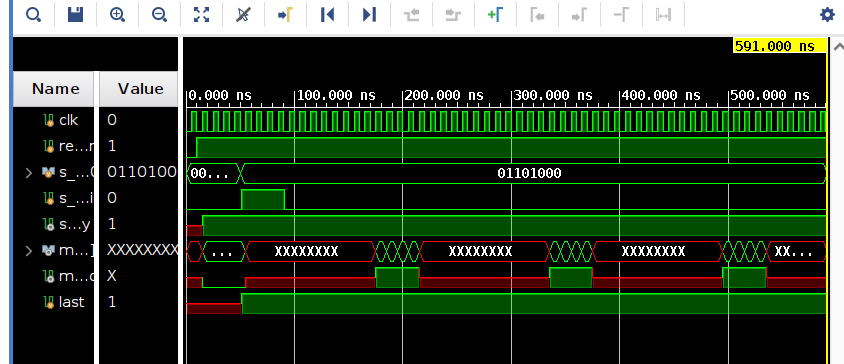
\includegraphics[width=\textwidth]{figs/p2rtlwavfull.png}
    \caption{Output of Verilog testbench}
    \label{fig:my_label}
\end{subfigure}
\hfill
\begin{subfigure}[b]{0.8\textwidth}
    \centering
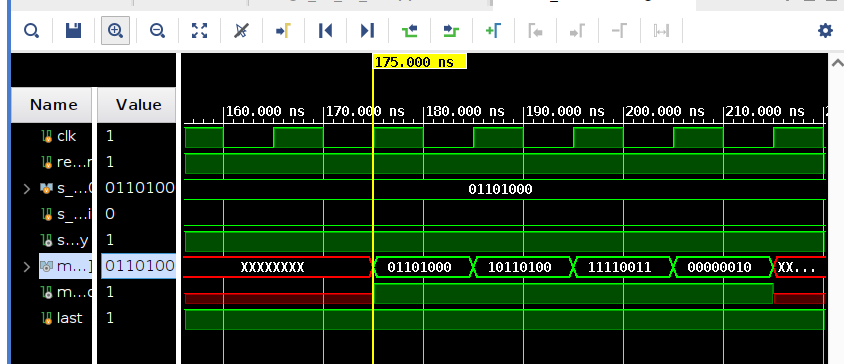
\includegraphics[width=\textwidth]{figs/p2rtlwav.png}
    \caption{Zoomed format of above figure}
    \label{fig:my_label}
\end{subfigure}
\end{figure}

\vspace{20cm}


\maketitle
\hfill \textbf{VIVADO-IP}
\section{Block Design}
\vspace{1cm}
\begin{figure}[h]
    \centering
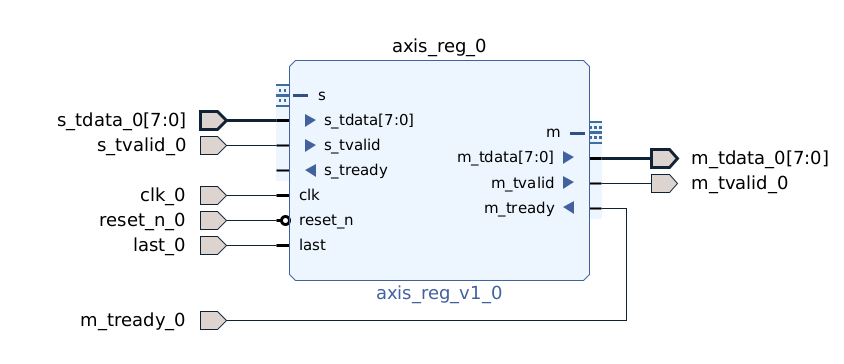
\includegraphics[width=\columnwidth]{figs/p2ipbd.png}
    \caption{Block Diagram}
    \label{fig:my_label}
\end{figure}
\vspace{13cm}
\section{Verilog Testbench}
\begin{lstlisting}
//axistb.v
`timescale 1ns / 1ps
//////////////////////////////////////////////////////////////////////////////////
// Company: 
// Engineer: 
// 
// Create Date: 06/27/2023 10:47:14 AM
// Design Name: 
// Module Name: axistb
// Project Name: 
// Target Devices: 
// Tool Versions: 
// Description: 
// 
// Dependencies: 
// 
// Revision:
// Revision 0.01 - File Created
// Additional Comments:
// 
//////////////////////////////////////////////////////////////////////////////////


module axistb(

    );
    reg clk;
    reg reset_n;
    reg [7:0] s_tdata;
    reg s_tvalid;
    wire s_tready;
    wire [7:0] m_tdata;
    wire m_tvalid;
    reg last;
    reg m_tready;
    
    // Instantiate the DUT (Design Under Test)
  /* axis_reg #(
        .DW_IN(8),
        .DW_OUT(32)
    ) dut (
        .clk(clk),
        .reset_n(reset_n),
        .s_tdata(s_tdata),
        .s_tvalid(s_tvalid),
        .s_tready(s_tready),
        .m_tdata(m_tdata),
        .m_tvalid(m_tvalid),
        .last(last)
    );*/
     design_rtl_IP_wrapper uut
   (.clk_0(clk),
    .last_0(last),
    .m_tdata_0(m_tdata),
    .m_tvalid_0(m_tvalid),
    .reset_n_0(reset_n),
    .s_tdata_0(s_tdata),
    .s_tvalid_0(s_tvalid),
    .m_tready_0(m_tready));
    
    // Clock generation
    always #5 clk = ~clk;
    
    initial begin
        // Initialize inputs
        clk = 0;
        reset_n = 1;
        s_tdata = 8'h00;
        s_tvalid = 0;
        
        
        // Apply reset
        reset_n <= 0;
        #10;
        reset_n <= 1;
        
        // Test scenario
        // Wait for reset to de-assert
        #40;
        
        // Send data and wait for it to be accepted
        s_tdata <= 8'b01101000;
        #1 last=1;
        
        s_tvalid <= 1;
        #40;
        s_tvalid <= 0;
        
        
        // Wait for some cycles
        #500;

        
        // Finish simulation
        $finish;
    end

endmodule


\end{lstlisting}

\vspace{15cm}


\section{Output Waveform}
\vspace{1cm}
\begin{figure}[h]
\centering
\begin{subfigure}[b]{1.1\textwidth}
    \centering
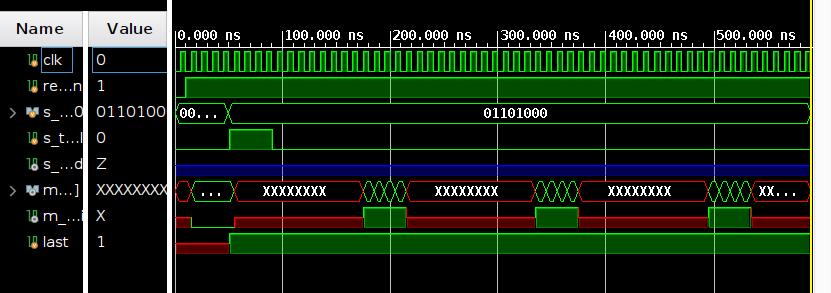
\includegraphics[width=\textwidth]{figs/p2ipwavfull.png}
    \caption{Output of IP testbench}
    \label{fig:my_label}
\end{subfigure}
\hfill
\begin{subfigure}[b]{1.1\textwidth}
    \centering
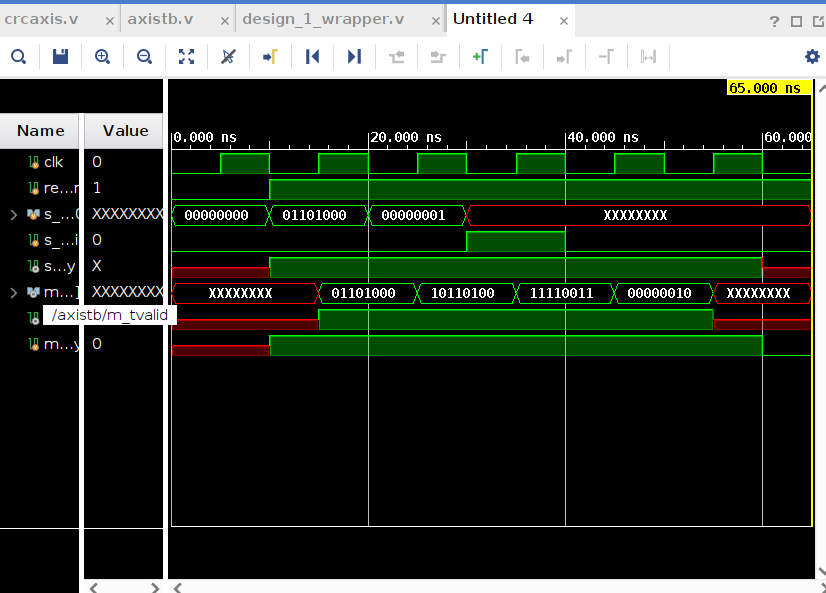
\includegraphics[width=\textwidth]{figs/p2ipwav.png}
    \caption{Zoomed format of above figure}
    \label{fig:my_label}
\end{subfigure}
\end{figure}
\vspace{15cm}

\maketitle
\hfill \textbf{MATLAB}
\section{Matlab Reference}
\begin{figure}[h]
\centering
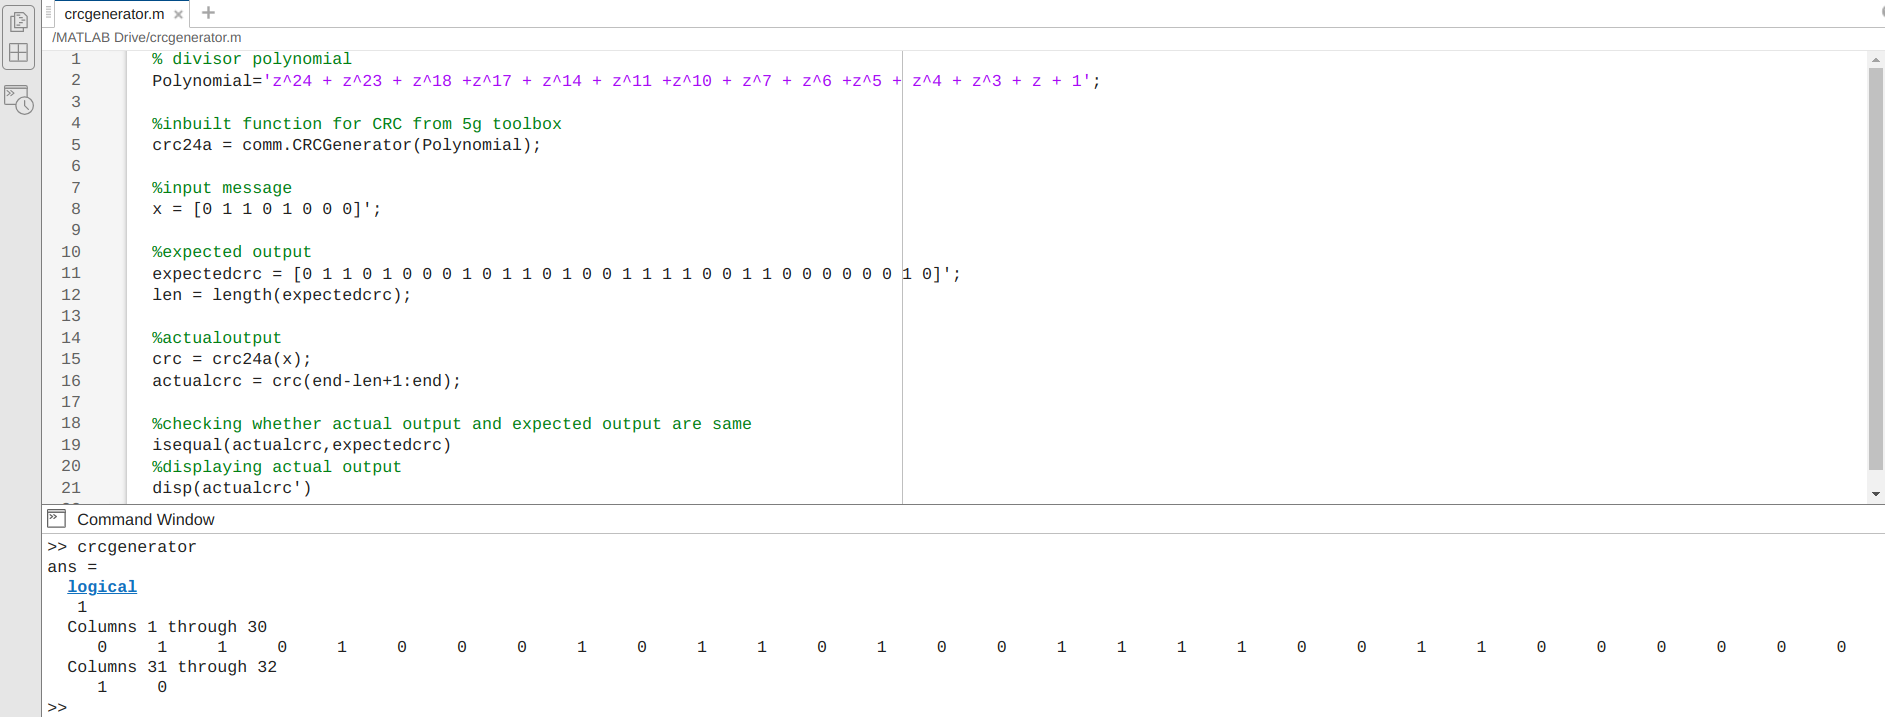
\includegraphics[width=1.3\textwidth]{figs/actual_matlab.png}
    \caption{Matlab Reference}
    \label{fig:my_label}
\end{figure}
\vspace{3cm}
\section{Conclusion}
\begin{lstlisting}
The Output of CRC IP is matching with Output of reference Matlab code and also
using this floating Point Converter Online :

\end{lstlisting}
\url{https://www.h-schmidt.net/FloatConverter/IEEE754.html}
\vspace{4cm}
\\
\textbf{GITHUB :} \url{https://github.com/dk-425/Training.git}
\end{document}


